\documentclass[english,12pt]{article}
\usepackage[T1]{fontenc}
\usepackage{geometry}
\geometry{verbose,bmargin=2.5cm,lmargin=2.5cm,rmargin=2.5cm}
\usepackage[utf8]{inputenc}
\usepackage{amsmath}
\usepackage{amsfonts}
\usepackage{amssymb}
\usepackage{rotfloat}
\usepackage{wasysym}
\usepackage{graphicx}
\usepackage{natbib}
\usepackage{latexsym}
\usepackage{caption}
\usepackage{flafter}
\usepackage{babel}
\usepackage{imakeidx}
\usepackage{amssymb,amsmath}
\usepackage[table]{xcolor}
\usepackage[mathlines,displaymath]{}
\usepackage{anyfontsize}
\usepackage{verbatim}
\usepackage{longtable}                                        
\usepackage{calc}                                             
\usepackage{multirow}                                         
\usepackage{hhline}                                           
\usepackage{ifthen} 
% \usepackage{babel}
\usepackage{tcolorbox}
\newtcolorbox{mybox}{colback=grey!5!white,colframe=red!75!black}
\usepackage{setspace}
\usepackage{verbatim}
\usepackage{etaremune}
\usepackage{url}
\usepackage{color}
\usepackage{graphicx}
\usepackage{natbib}
\usepackage[latin1]{inputenc}
\usepackage{color}
\usepackage{array}
\usepackage{float}
\usepackage{wrapfig}

\newcommand{\etal}{{et~al.{}}}
\newcommand{\ie}{{i.~e.{}}}
\newcommand{\eg}{{e.~g.{}}}
\newcommand{\viz}{{viz.{}}}
\newcommand{\etc}{{etc.{}}}
\newcommand{\apriori}{{a priori{}}}
\newcommand{\vv}{{vice versa{}}}
\newcommand{\cf}{{}}
\usepackage{titling}
\usepackage{color}
\usepackage{subfigure} 

\date{}

\topmargin 0.0cm
\oddsidemargin 0.5cm
\evensidemargin 0.5cm
\textwidth 16cm 
\textheight 22cm

\makeindex
\begin{document}
\begin{flushleft}
  \textbf{\Large Distributed Open Automated Research Platform\\
    \\
    \vspace{0.5cm}
    $\mathcal{ROBHOOT}$}\\
  \\
  \\
  \vspace{0.5 in}
  {\bf Current Team:}\\
  \\
    Carlos J. Meli\'an\textsuperscript{1} Switzerland C1\\
    Victor Egu\'iluz\textsuperscript{2} Spain C2\\

    {\bf Tentative Team:}\\
    Swiss Science Data Center\textsuperscript{3} Switzerland C1\\
    Eawag IT (Harald)\textsuperscript{4} Switzerland C1\\
    iDiv IT ()\textsuperscript{5} Germany C3\\
    Inca (Nterminal, Yupana)\textsuperscript{6}\\
    Benoit Baudry (DIVERSIFY-project)\textsuperscript{7} France C4

  
%Ali R. Vahdati\textsuperscript{1, *}\\
%Charles N. de Santana\textsuperscript{2}\\
%Alejandro Rozenfeld\textsuperscript{3}
  \vspace{0.5cm} 
%\textbf{1} Department of Anthropology, University of Zurich, Switzerland\\
%\textbf{2} Institute of Evolutionary Biology and Environmental Studies, University of Zurich, Switzerland\\
%\textbf{3} Conicet-cificen-intelymec, University of the Center of Buenos Aires, Argentina\\
  \textbf{1} Eawag Center for Ecology, Evolution and Biogeochemistry, Switzerland\\
  \textbf{2} Inst. de Física Interdisciplinar y Sistemas Complejos, IFISC\\
  (CSIC-UIB), Palma de Mallorca, Spain.\\
  \textbf{3} Tentative team
\\
\bigskip
\end{flushleft}
\newpage




\tableofcontents
\newpage

\begin{comment}
\section{Funding scheme A}

\begin{mybox}\begin{singlespace}
 {\bf{Call ID: FET Proactive: emerging paradigms and communities\\ H2020-FETPROACT-2019-2020}}\\
 \begin{small}
   {\bf Specific Challenge}:\\
   To explore and consolidate a new technological direction in order
   to put it firmly on the map as a viable paradigm for future
   technology. To foster the interdisciplinary communities that are
   able to drive this forward, extending from the participating
   consortia to a wider European pool of expertise. To stimulate the
   emergence of a European innovation eco-system around a new
   technological paradigm, well beyond the world of research alone.\\
   \\
   {\bf Scope}:\\
   Proposals are sought for cutting-edge high-risk / high-reward
   research and innovation projects that aim to demonstrate a new
   technological paradigm within the scope of one of the following
   sub-topics:\\
   \\
   {\bf Human-Centric AI}. Artificial intelligence (AI) is gaining more and
   more footholds in various aspects of our life. However, machine
   learning algorithms are difficult to understand, opaque and may
   have implicit biases in their decision making. Explicability has
   become an essential element if users are to trust, accept and adopt
   the next generation of intelligent machines on a wider scale. This
   initiative seeks to advance to the next AI frontier with
   verifiable, evidence-based features of trustworthiness (i.e.,
   reliable and unbiased alignment of values, goals and beliefs) and
   transparency (explainable performance), exploring radically new
   approaches (e.g., inspired from neuro-science, cognition or social
   science). For instance, explanation could be more tightly
   intertwined with the decision making process itself so that
   decisions can be challenged, interpreted, refined and adjusted
   through mutual exchange, introspection (e.g., self-awareness of
   biases, reflecting on the internal functioning of the learning
   system, or on what caused a wrong or unacceptable decision) and
   active learning of both system and user, for example through
   dialogue or other forms of multi-modal interaction aimed at
   establishing mutual trust. New data collection and
   ownership/governance models that go beyond the dominant off-line
   and centralised data processing should be investigated, and new
   avenues, such as for incremental, unsupervised, active, one-shot
   and ‘small data’ machine learning, should be explored. The projects
   are expected to contribute to the wider debate on the
   sociotechnical, organisational and AI-ethical dimensions of such
   technologies and systems, and link to the ’Commission’s broader AI
   strategy
   \\
   {\bf Deadline}: September 3, 2019 12:30:00 AM The submission session is now
   available for: FETPROACT-EIC-05-2019(RIA),
   FETPROACT-EIC-06-2019(RIA)

\end{small}
\end{singlespace}
\end{mybox}

\end{comment}

\newpage
\section{Funding scheme}

\begin{mybox}\begin{singlespace}
 {\bf{Call ID: FET-Open Challenging Current Thinking\\ H2020-FETOPEN-01-2018-2019-2020}}\\
 \begin{small}
   {\bf Specific Challenge}:\\
   To lay the foundations for radically new future technologies of any
   kind from visionary interdisciplinary collaborations that dissolve
   the traditional boundaries between sciences and disciplines,
   including the social sciences and humanities. This topic also
   encourages the driving role of new actors in research and
   innovation, including excellent young researchers, ambitious
   high-tech SMEs and first-time participants to FET under Horizon
   2020 from across Europe.\\
   \\
   {\bf Scope}:\\
   Proposals are sought for cutting-edge high-risk / high-impact
   interdisciplinary research with all of the following essential
   characteristics ("FET gatekeepers"):
   \\
   {\bf Radical vision}: the project must address a clear and radical
   vision, enabled by a new technology concept that challenges current
   paradigms. In particular, research to advance on the roadmap of a
   well-established technological paradigm, even if high-risk, will
   not be funded.
   \\
   {\bf Breakthrough technological target}: the project must target a novel
   and ambitious science-to-technology breakthrough as a first proof
   of concept for its vision. In particular, blue-sky exploratory
   research without a clear technological objective will not be
   funded.\\
   \\
   {\bf Ambitious interdisciplinary research} for achieving the
   technological breakthrough and that opens up new areas of
   investigation. In particular, projects with only low-risk
   incremental research, even if interdisciplinary, will not be
   funded.
   \\
   The inherently high risks of the research proposed shall be
   mitigated by a flexible methodology to deal with the considerable
   science-and-technology uncertainties and for choosing alternative
   directions and options.
   \\
   The Commission considers that proposals requesting a contribution
   from the EU of up to EUR 3 million would allow this specific
   challenge to be addressed appropriately. Nonetheless, this does not
   preclude submission and selection of proposals requesting other
   amounts.
 \\
   {\bf Expected Impact}: \\
   Scientific and technological contributions to the foundation of a
   new future technology Potential for future social or economic
   impact or market creation.  Building leading research and
   innovation capacity across Europe by involvement of key actors that
   can make a difference in the future, for example excellent young
   researchers, ambitious high-tech SMEs or first-time participants to
   FET under Horizon 2020.
   \\
   {\bf Deadline}: ID: September 18, 2019 17:00:00 Brussels time
   FETOPEN-01-2018-2019-2020
\end{small}
\end{singlespace}
\end{mybox}

\newpage

\section{Excellence}
Public funded data is the norm in science and engineering
landscapes. Yet, distributed and open-source automated
knowledge-inspired technology accounting for the interdisciplinary
research cycle remains challenging in science and engineering. We
propose a decentralized automated research platform to facilitate
reproducibility in a knowledge-inspired society, technology and
science. The platform will be implemented in two stages. First, a
testnet biodiversity research prototype accounting for data
integration and inference to visualization and reporting
generation. Second, a mainnet platform integrating literature
discovery, data integration, inference, validation, visualization and
reporting generation. Decentralized and open automated research
platforms can strongly contribute to a knowledge-inspired governance
to help take informed decisions in solving complex social problems
merging interdisciplinary science and technology.
\\
\\
Keywords: Knowledge-inspired society, Data integration, Multilayer
networks, Deep explicability-based learning, Transparent governance,
Bayesian inference. Probabilistic Bayesian networks.
\newpage

\subsection{Radical vision of a science-enabled technology}

\begin{comment}
Describe the vision of a radically-new science-enabled technology that the project 1
would contribute towards.

• Describe how this vision surpasses substantially any technological
paradigms that currently exist or are under development.

• Describe the overall and specific objectives for the project, which
should be clear, measurable, realistic and achievable within the
duration of the project. (The details of the project plan belong to
the Implementation section).
\end{comment}


Decentralized, open and scalable automated research platform
accounting for a fully interdisciplinary research cycle, from
hypothesis tracking, literature and data
integration to inference, visualization and reporting generation.\\



\subsection{State of the art}
\\
\\
\begin{mybox}\begin{singlespace}
 {\bf{}}\\
 \begin{small}
   {\bf Radical vision:}\\
   \begin{itemize}
  
   \\
   {\bf Breakthrough technological target:}\\
    \begin{itemize}
    \item Transparent automated data-rule-knowledge-inspired technology fully
   accounting for the interdisciplinary research cycle.
    \end{itemize}
   \\
   {\bf Ambitious interdisciplinary research:}\\
   \begin{itemize}
   \item Mixing researchers, engineers and society to build an open
     and transparent data-rule- and knowledge-inspired science,
     technology and society.
   \end{itemize}
   \\
\end{small}
\end{singlespace}
\end{mybox}


\begin{mybox}\begin{singlespace}
 {\bf{}}\\
 \begin{small}
-------------How to solve it?---------\\
1. The problem:\\
       Why? Centralized, Non-transparent and non-reproducible vs decentralized, transparent and reproducible\\
       Is it radikal?\\
       Is it viable? Efficient?\\
       Which are the Knowns?\\
       Unknowns? \\
2. Our own plan\\
       How much time?\\
       Existing gaps? Why?\\
       Data available? Methods? Main gaps\\
       Our own method? Why?\\
3. Carry on the plan\\
       Quantitative assessment\\
       The maths\\ 
4. Solutions (Milestones) \\
5. Go backwards (Reproducibility)\\
   Is it correct? Reproducible? Scalable? Decentralized? Safe?\\
   Apply to other problems? Datasets?\\
-------------------------------------
\end{small}
\end{singlespace}
\end{mybox}

\newpage

%Communication of...
%
%The tradeoffs among data-, rule- and knowledge-inspired technology...
%\\
%Bias, uncertainty and automation of the whole scientific cycle to
%target knowledge-inspired technology, science and society...

%For example... \\
Automation is rapidly occurring in many fronts, from robotics and
investments to gaming and ecommerce. Many technologies are in a era of
massive data accumulation, integration and pattern detection. Yet,
obtaining insights from such an integration accounting for open
science, full reproducibility, inference and prediction power is at a
very incipient stage \citep{Ioannidis2005,Reichsteietal2019}. There
are many challenges when aiming to integrate data, inference and
prediction. For example, sampling design and experiments \index{robust
  experiments} \citep{Voelkl2018}, randomizations to achieve solid
statistics \index{robust algorithms}, and process- or pattern-based
model selection and inference \index{robust inference} just to name a
few. All these steps require many intermediate decisions that make the
scientific process challenging to decentralize, repeat, replicate, and
reproduce. Currently, there are many protocols and platforms
automatizing partial steps of the \index{research cycle} (Table 1
summarize a non-exhaustive list of automated platforms).

Reproducibility, robustness and minimizing bias across the different
stages of a research platform are two of the desire properties of
automated research platforms. Reproducibility guarantees the future
improvement of the results and many programming languages currently
offer tools to facilitate reproducibility (i.e., Jupyter
notebooks). Automated research platforms will facilitate tracking the
explored paths (i.e., the within and between layer interactions,
Figure 1) and can produce statistics on how close each path is to the
empirical patterns.

The following are six features of open automated research platforms
\index{Open automated research platforms} that might play a leading
role in moving towards a information-inspired science, society and
technology: 1) Building the science of science to provide quantitative
statistics
% \citep{Fortunatoeaao0185}
of interdisciplinary science (Figure 1 for the arquitecture of an
automated research platform); 2) Identifying systematically and
accounting for bias and uncertainty in inference; 3) Exploring
prediction and explanatory gradients to gain sinergy between AI
predictive approaches and explanatory power to complex problems
(Figure 2); 4) Identifying gaps in patterns not explored consequence
of lack of syntesis in interdisciplinary research, 5) Allowing for
reusability, repeatibility, replicability and reproducibility along
the many paths in the scientific enterprise, and 6) Building on
rapidly evolving open-source computing programming languages to
facilitate the decentralization, scalability and integration of the
scientific process (Table 2 and Figure 3).


%The design or
%research platforms is still in its infancy. Many factors are involved
%in research platforms: the programming language, the number of
%packages and their interactions, their efficiency and functionality,
%etc... Pros and cons automated research platforms

%data-rule-knowledge-inspired technology, society and science (Figure 2)...\\
%One of the most discussed challenges nowadays is how to balance
%pattern and process inference. Many problems might not require a
%mechanistic understanding to make predictions. Recent examples are AI
%algorithms playing chess and go using brute force or rules based
%algorithms (refs). They do not require a theory of mind to win. On the
%other side, there can be problems that might require a solid
%mechanistic understanding to make more accurate predictions or to take
%better informed decisions. Examples of these problems can be global
%warming or astrophysics. Therefore platforms that learn to combine AI
%and process-based methods can be used to have quick overviews of
%the...
%Example and results exploring PI vs TI gradient -- PI, TI or hybrid PTI 

%Prototyping an ARP, which programming language?
%Discuss prototype (Figure 3)

\begin{comment}
\section{Prototyping a decentralized and open automated research
  platform}

Communicate the full universal cycle of scientific research...\\
Which are the minimum number of layers that would be needed to develop an interdisciplnar ARP?\\
Check Figure 1, data collection and integration, complexity reduction,
pattern-process inference, validation and
visualization.\\
\\
\\
Introduce the features of a simple prototype, the $\mathcal{ROBHOOT}$
ARP.
\\
\\
General vision of ARP\\
The science of science ARP. For example, for any given question, there
are different methods within each layer that can complete the
task. Ideally, one should be able to choose the best method from each
layer and connect them to reach insightful patterns and predictions
from the data. How many paths are there?  Which of these minimize
bias? Which topology within and between layers give the best response
to our question?

\begin{mybox}\begin{singlespace}
 {\bf{Research cycle in Automated Research Platforms}}\\
 \begin{small}
\subsection{Data Integration}
Databases in many fields currently have multiple examples of
duplicated systems. In addition, datasets are currently highly
scattered across many distinct platforms and protocols making
difficult to researchers and the public to hace access to the data
while dealing with a highly complex set of intermediate stages and
regulations before having access to the raw data. Data shared ledgers
(refs) including replication by participans will facilitate data
access and integration across research platforms (refs). Distributed
technologies to unify many distinct datasets sharing minimal
information are rapidly evolving (i.e., hyperledger fabric, Ethereum)


is rapidly evolving and there are many
platforms that can have access and deliver real time data plots (Table
1).

To be added to the outlining of the ARP\\
Data Integration and standarization -- Size effects -- N labs vs N
samplings per lab: Accuracy and uncertainty: How do initial
distributions change accuracy and uncertainty? Trade-offs experimental
vs big data

\subsection{Complexity Reduction}
\subsection{Pattern-Process Inference}
\subsection{Validation}

Describe briefly Bayesian Inference, Approximate Bayesian computation,
AIC and BIC model comparison methods.  Gibbs sampling -- Bayes factors

\subsection{Visualization}
\end{small}
\end{singlespace}
\end{mybox}


\begin{comment}
PCA family -- High-dimensionality of Convex hull -- Information metrics multilayer networks\\


Data dimension reduction is a second step to increase performance
during the next stages of analysis.  Complexity reduction in economics
and in ecology has a long tradition mostly by looking at
variance-covariance matrices.  Portfolio theory in economics has a
long tradition \citep{MarkowitzBook}. The theory is rooted in the
concept of efficient frontier\index{efficient frontier}. There are
several packages in several languages to calculate efficient
frontiers\footnote{\url{http://www.quantcode.com/}}$^{,}$\footnote{\url{https://github.com/JuliaQuant/PortfolioModels.jl}}$^{,}$\footnote{\url{https://www.wikinvest.com/account/portfolio/register}}$^{,}$\footnote{\url{https://d1so5k0levrfcn.cloudfront.net/SigFig\%20Investment\%20Methodology.pdf}}. Most
maths underlying portfoliio theory\index{portfolio theory} are based
in matrix correlation patterns\index{matrix correlation patterns}. In
ecology, portfolio concept has also been used to predict the number of
coexisting species in landscapes with highly fluctuating
environments\footnote{Check references}.

Many fields aim at predicting fluctuations of several time series at
local and regional scales. The better the predictions are the better
we know the ecosystem. Unfortunately, it is not easy to predict time
series of a large number of interacting (ideally independent)
variables. Given we can not predict most of the ideas' trends, we
should build a minimum understanding on how to investigate ideas and
build a diversified portfolio with a balance between risk and
reward. Basic questions will always remain when discussing about
predicting the future and diversifying portfolios. For example, in a
complex ecosystem, which is the best strategy under complete
ignorance? And under complete information?  Should we invest in ideas
following a random walk \index{random walk}? Should we produce a
portfolio with neutral risk \index{neutral risk}?
\footnote{\url{https://en.wikipedia.org/wiki/A$_$Random$_$Walk$_$Down$_$Wall$_$Street}}. Given
the basic maths underlying complexity reduction, which are the
algorithms and models out there? Which one perform the best? Which is
the mixed of models to minimize data complexity?
\\
\end{comment}


\end{comment}

\section{Milestones}

\subsection{Milestone 1: $\mathcal{ROBHOOT}$ testnet}
Building a functional testnet case for an automated research
platform. We will use a Biodiversity research case for this testnet as
a showcase of how to gain insights about knowledge-inspired technology
(See Robhoot testnet box).

\begin{mybox}\begin{singlespace}
    {\bf{$\mathcal{ROBHOOT}$ testnet}}\\
    Develop automated packages for each layer (See Figure 3 and Table
    2 for a prototype in the computing language Julia. The platform
    will have access to data from both centralized and decentralized
    platforms in Biodiversity research
    \footnote{\url{https://github.com/melian009/Robhoot/blob/master/resources/databases.md}}
    .
 \begin{small}
\subsubsection{Milestone 1.1: Data Integration ($\mathcal{DAADI}$)}
%Automated package combining access to data from both centralized and
%decentralized platforms in Biodiversity research
%\footnote{\url{https://github.com/melian009/Robhoot/blob/master/resources/databases.md}}
%to create an integrated databases (Figure 3 and Table 2).

\subsubsection{Milestone 1.2: Complexity Reduction ($\mathcal{GOCORE}$)}

\subsubsection{Milestone 1.3: Pattern-Process Inference ($\mathcal{PROPENCE}$)}
  
\subsubsection{Milestone 1.4: Validation ($\mathcal{VATION}$)}

\subsubsection{Milestone 1.5: Visualization ($\mathcal{VITION}$)}

\end{small}
\end{singlespace}
\end{mybox}

\subsection{Milestone 2: $\mathcal{ROBHOOT}$ mainnet}
Develop a platform fully integrated in decentralized network platforms \footnote{\url{https://golem.network/}}

%Scalability\\
%Security \\

\begin{mybox}\begin{singlespace}
 {\bf{$\mathcal{ROBHOOT}$ mainnet}}\\
 \begin{small}
\subsubsection{Milestone 2.1: Data Integration}

\subsubsection{Milestone 2.2: Complexity Reduction}

\subsubsection{Milestone 2.3: Pattern-Process Inference}
  
\subsubsection{Milestone 2.4: Validation}

\subsubsection{Milestone 2.5: Visualization}

\end{small}
\end{singlespace}
\end{mybox}


%\section{Deliverables}


%\newpage
%\section{Budget}


\newpage
\bibliographystyle{evolution}
\bibliography{ref}

\newpage

\section{Tables}
\begin{center}
\rowcolors{1}{white}{pink!50}
\begin{tabular}{  p{5cm}  |  p{8cm} }
%\bottomrule
\hline
{\bf Table 1} & \textbf{}\\  \hline
  \textbf{Automated platforms} & \textbf{Webpage}\\  \hline
        Nakamoto Terminal & https://www.nterminal.com \\ \hline
        BigQuery & https://cloud.google.com/bigquery/ \\ \hline
        Automated statistician  & https://www.automaticstatistician.com/index/ \\ \hline
        Modulos & http://www.modulos.ai/ \\ \hline
        Google AI & https://ai.google/ \\ \hline        
        Iris & https://iris.ai \\ \hline
         & \\ \hline 
         & \\ \hline        
         & \\ \hline
         & \\ \hline
         & \\ \hline
         & \\ \hline
         & \\ \hline
         & \\ \hline
         & \\ \hline
         & \\ \hline
        
\bottomrule
\end{tabular}
\end{center}

\newpage

\begin{mybox}\begin{singlespace}
 {\bf{Table 2: Prototyping a script workflow in $\mathcal{ROBHOOT}$}}\\
 \begin{small}
   \\
   SUMMARY==========================================
   This is a prototype for a script workflow to automate interactions among data search, parsing, integration, database, cleaning, data complexity reduction, pattern and process inference, validation and visualization. The script is based in two types of packages: backbone and specialized packages. Backbone packages (B) connect intra- and inter-layer algorithms to automatically run the workflow. Specialized (S) packages feedback with backbone packages to run specific tasks: parsing, likelihoods, inference, plotting, visualizing, etc. \\

================================================
 \\
Layers========================\\
DATA INTEGRATION: D \\
COMPLEXITY REDUCTION: C \\
PATTERN-PROCESS INFERENCE: P \\
VALIDATION: VA \\
VISUALIZATION: VI \\
==============================
 \\
EXAMPLE with julia ============= \\
Julia packages: \\
https://github.com/melian009/Robhoot/blob/master/packages.md \\
 \\
WORKFLOW NETWORK----------------------------- \\
 \\
data.search D S                $------>$ Retriever.jl {\bf M1} \\
parsing.data D S               $------>$ Query.jl  {\bf M1} \\
data.to.table D S              $------>$ MySQL.jl SQLite.jl Clickhouse.jl {\bf M1} \\
data.julia D S                 $------>$ DataFrames.jl {\bf M1} \\
table.comp.reduction C B       $------>$ TensorFlow.jl lm4.jl Clustering.jl OnlineAI.jl LightGBM.jl \\
pattern.detection P S          $------>$ TensorFlow.jl DataVoyage.jl DataFitting.jl Mocha.jl DeepQLearning.jl Flux.jl AnomalyDetection.jl \\
proccess.simulation P S        $------>$ Simjulia.jl Agents.jl JuliaDynamics.jl Zygote.jl \\
pat.proc.infer P S             $------>$ mads.jl temporal.jl GlobalSearchRegression.jl BlackBoxOptim.jl JuMP.jl GeneticAlgorithms.jl NaiveBayes.jl Mamba.jl ABC.jl ApproxBayes.jl DynamicHMC.jl \\
validation.pat.proc VA S       $------>$ mads.jl LearningStrategies.jl Mamba.jl ABC.jl Measurements.jl \\
visualiztion.pattern.process   $------>$ Makie.jl VegaLite.jl \\
\end{small}
\end{singlespace}
\end{mybox}


\newpage

\section{Figures}

\vspace{-7 in}
%Fully connected layers and a specific example
\begin{figure}
  \vspace{-7 in}
\begin{center}
  \hspace{-0.5 in}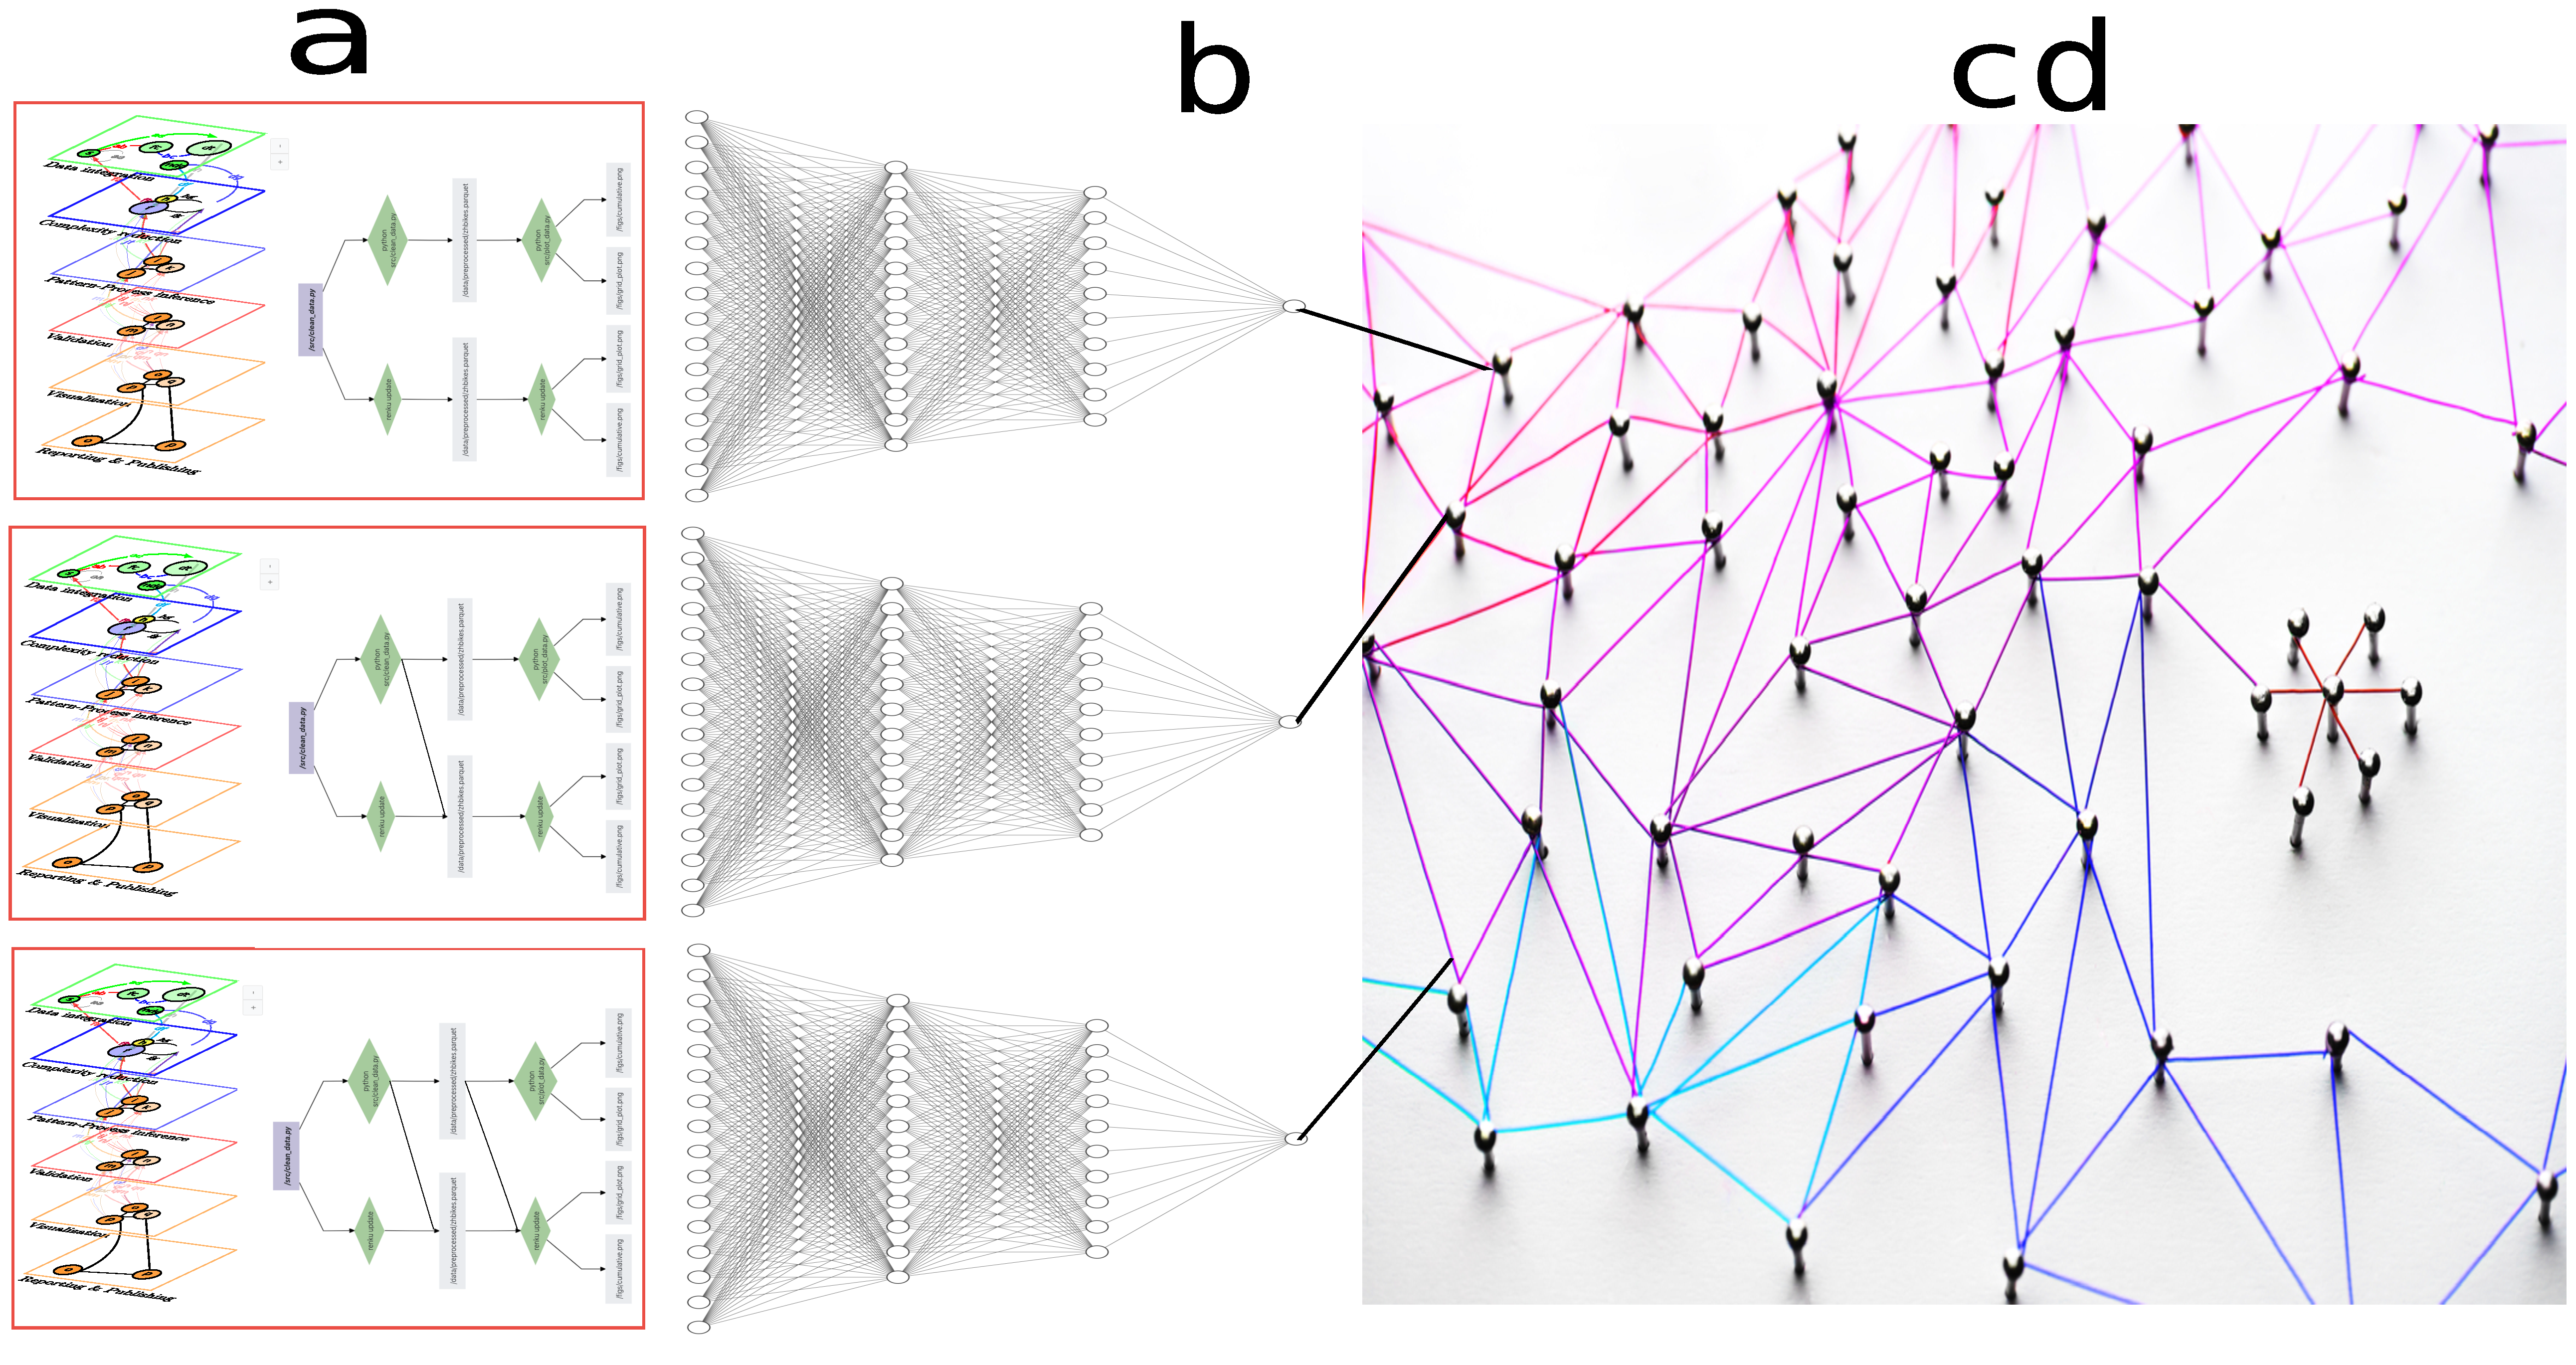
\includegraphics[width=9cm,height=14cm]{Figure1.pdf}\\
\end{center}
\caption{A cartoon of a five layer automated research platform: Data
  Integration, Complexity reduction, Pattern-process inference,
  Validation, and Visualization. Nodes and links represent algorithms
  and interactions between two algorithms, respectively. For example,
  the figure shows five algorithms in the layer Data integration
  ({\bf a}, {\bf b}, {\bf c}, {\bf d}, and {\bf e}). Algorithm {\bf a}
  interacts with algorithm {\bf b} and {\bf e} in the same layer
  (intra-layer connections) and with algorithm {\bf f} from the second
  layer (inter-layer connection), Complexity reduction. The cartoon
  represents many intra- and inter-layer connections to solve a
  problem. The paths can be quantified by many metrics each producing
  a distribution of automated solutions. This distribution can be
  analyzed with the ones used for a specific domain in science, the
  science of science of a domain, to quantify properties as
  robustness, reproducibility and bias of a domain.}
\label{}
\end{figure}

\newpage


\begin{figure}
\begin{center}
  \hspace{-0.5 in}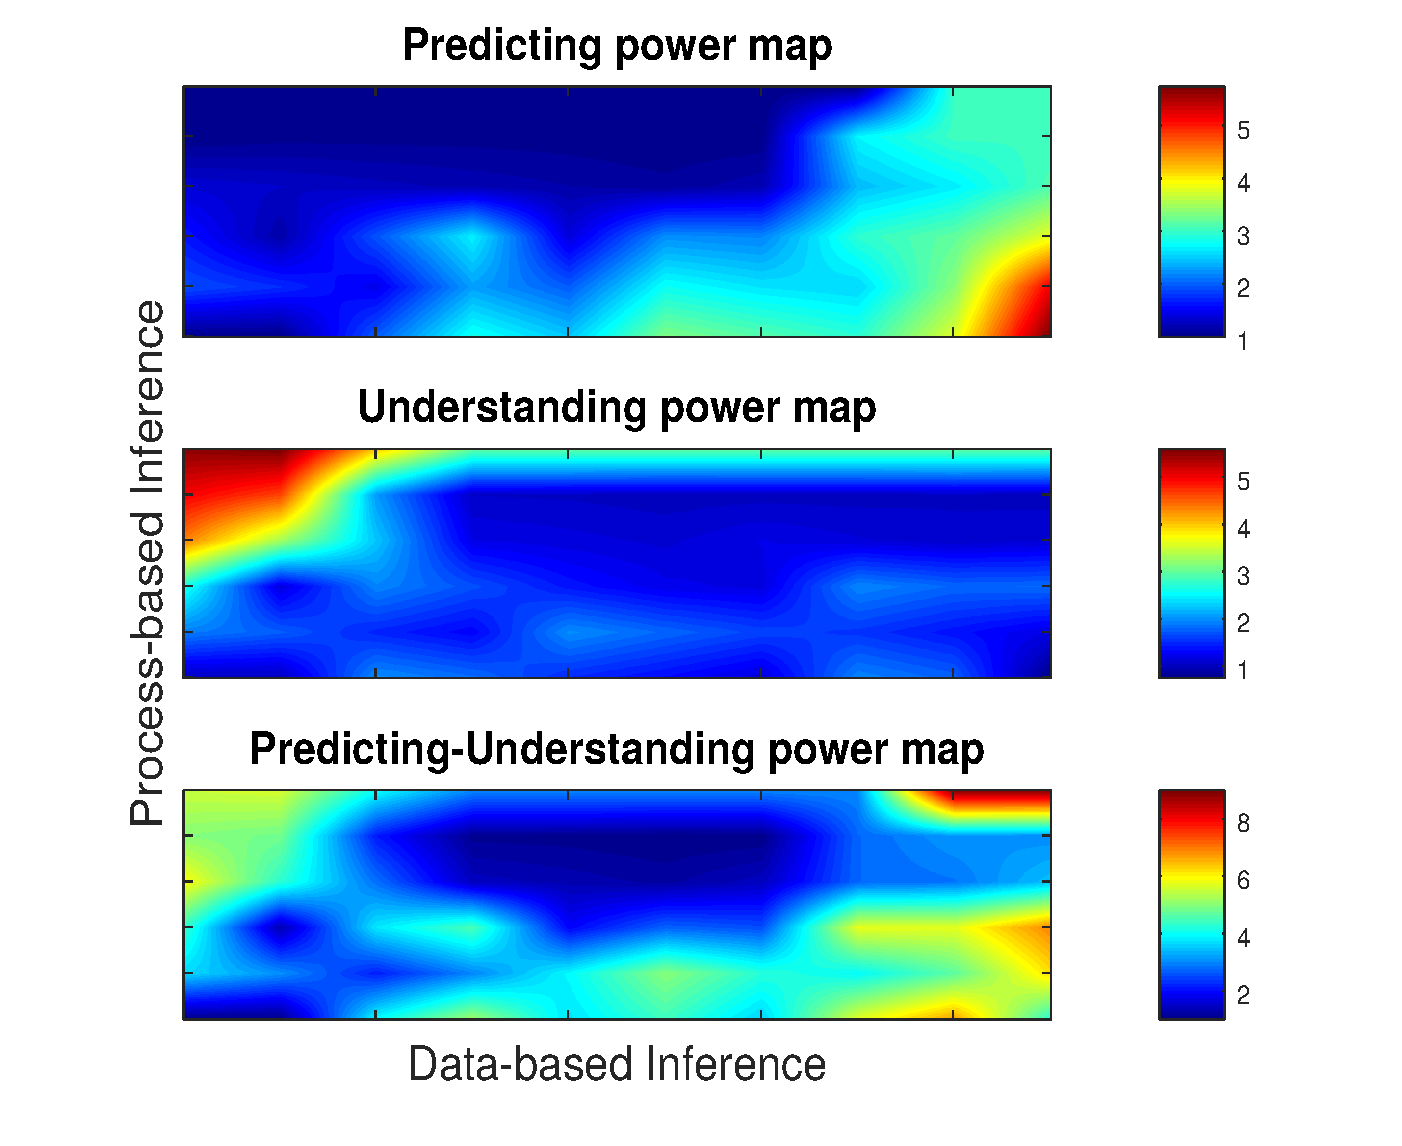
\includegraphics[width=16cm,height=16cm]{Figure3.pdf}\\
\end{center}
\vspace{-0.25 in}
\caption{Predicting and knowledge power can be joined to drive open
  knowledge-inspired societies, technology and science. This figure
  shows a cartoon of the predicting power (top), the knowledge power
  (middle), and the predicting-knowledge power (bottom). x- and y-axis
  represent data-based inference (i.e., gradient of AI methods from
  low (left) to high (right) predictive power) and process-based
  inference (i.e., gradient of process-based methods from low (bottom
  left) to high (top left) knowledge power). The gradient of
  predicting power (top) shows a hot spot red area in the bottom right
  highlighting the region where AI methods best predict any given
  empirical data. The gradient of knowledge power (middle) shows a hot
  spot red area in the top left highlighting the region where the best
  mechanistic understanding of a problem occur. The
  predicting-knowledge power (bottom) integrates the sum of the two
  previous maps highlighting a red hot spot where interdisciplilnary
  research joining predicting and knowledge power of the empirical
  data occur.}
\label{}
\end{figure}

\newpage
\begin{figure}
\begin{center}
\hspace{-0.5 in}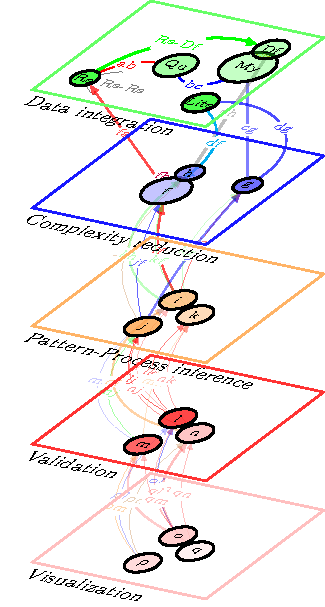
\includegraphics[width=9cm,height=14cm]{Figure2.pdf}\\
\end{center}
\caption{A julia prototype of an automated research platform. Nodes
  and links in each layer represent julia packages and interactions
  between two packages, respectively. The figure shows julia packages
  within each layer. For example, the layer Data integration contains
  the packages "Retriever.jl" ({\bf Re}), "Query.jl" ({\bf Qu}),
  "MySQL.jl" ({\bf My}), "SQlite.jl" ({\bf lite}), and "DataFrames.jl"
  ({\bf df}). }


%Algorithm \bf{a} interacts with algorithm \bf{b} and \bf{e} in the
%same layer (intra-layer connections) and with algorithm \bf{f} from
%the second layer (inter-layer connection), Complexity reduction.

%The cartoon represents many intra- and inter-layer connections to
%solve a problem. The paths can be quantified by many metrics each
%producing a distribution of automated solutions. This distribution can
%be analyzed with the ones used for a specific domain in science, the
%science of science of a domain, to quantify properties as robustness,
%reproducibility and bias of a domain.  }
\label{}
\end{figure}

%\newpage
%\begin{figure}
%\begin{center}
%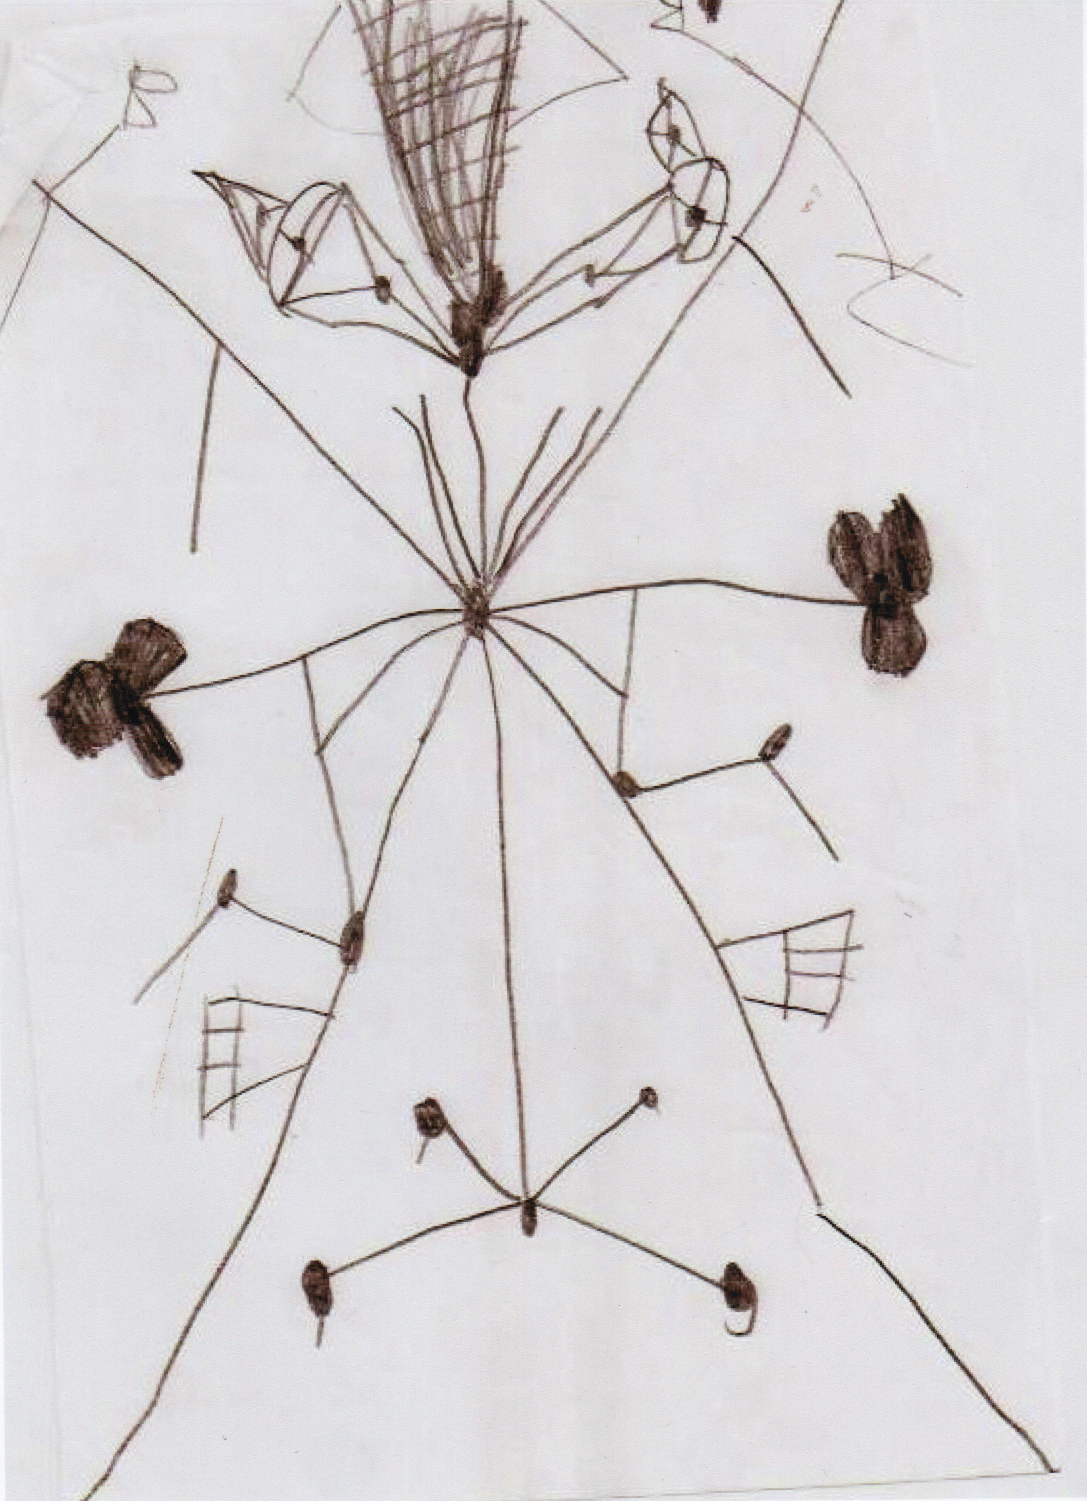
\includegraphics[scale=0.4]{robhootcartoon.pdf}
%\end{center}
%\caption{$\mathcal{ROBHOOT}$} -- An open multilayer platform for data integration, inference and prediction}
%\end{figure}
%\newpage



\newpage

%\begin{figure}
%\vspace{-1 in}
%\begin{center}
%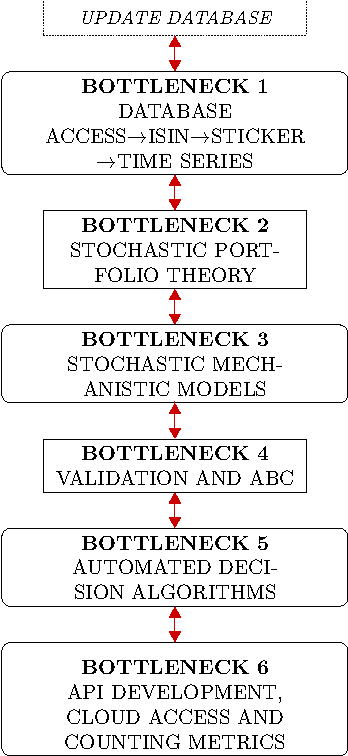
\includegraphics[scale=1.25]{EasyFlowChartBottlenecks.pdf}
%\end{center}
%\caption{Packages graph in $\mathcal{ROBHOOT}$: Visualization: Julia(Tikz and Tikz-network)}
%\end{figure}
%\newpage


\printindex
\end{document}
